\section{Proposal}

With Swift, the available access control mechanism is  ACL (Access Control List) which specifies who can or cannot access an object or a file. In this approach, if someone can access a document, he/she gets the full content of the document which is an all-or-nothing approach.  Figure \ref{fig:swiftfile} and \ref{fig:zwiftfile}  illustrates the situation where in the former case, a file is accessed in all-or-nothing approach and in the later case the file can be selectively accessed by different users. But we believe that   ZeroVM enables more sophisticated cases which require more flexible access control than the ACL. For example,  a hospital that stores patient medical records in the cloud,  wants all its doctor, nurse or patient access selective content based on the available role of the requester.  So, along with the content, the owner (in this case, the hospital) of an object/file may need to specify who can access how much of the content.

\begin{figure}[h!] 
  \centering
    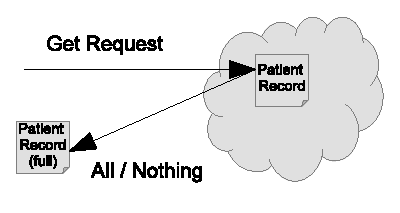
\includegraphics[width=0.3\textwidth]{eps/swift_file}
 \caption{Accessing file with Swift API.}
\label{fig:swiftfile}
\end{figure}

\begin{figure}[h!]
  \centering
    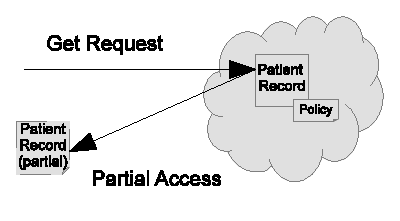
\includegraphics[width=0.3\textwidth]{eps/zwift_file}
 \caption{Our Proposed Solution where file can be accessed selectively}
\label {fig:zwiftfile} 
\end{figure}




Figure  \ref{fig:patient Record}, shows a sample file to be stored in the object store. For our example, we specify following different user roles namely, doctor, patient, nurse and billing stuff.
A sample policy to be specified by the content owner is shown below.

\begin{figure}[h!]
  \centering
    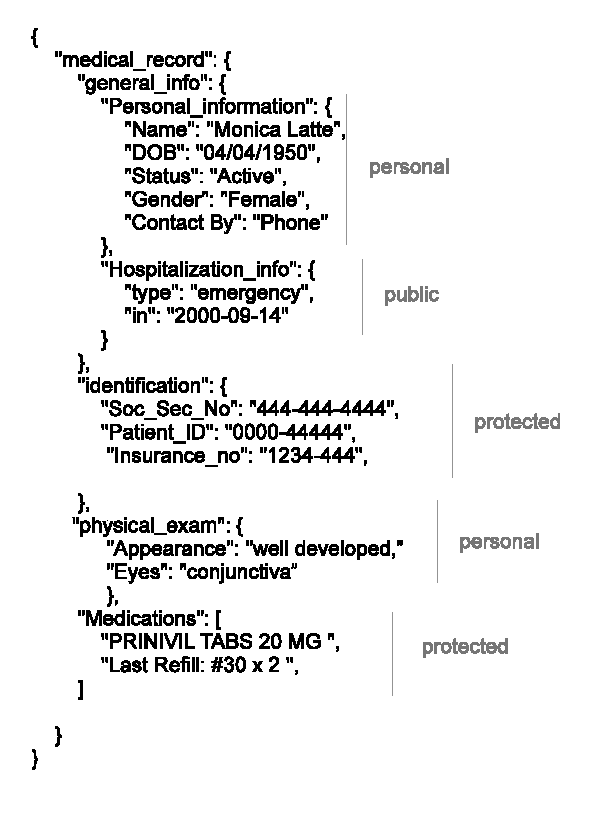
\includegraphics[width=0.3\textwidth]{eps/json-data}
 \caption{Labeled JSON data.}
\label {fig:patient Record} 
\end{figure}



\begin{enumerate}

  \item   Patient own 'personal\_Information' and 'physicalExam' records (see Fig. \ref{fig:patient Record} ). Only the owner can read it.

\item  Patient allow doctor to read her 'physicalExam' records  .
\item  Doctor can read  the entire medical records except information owned by the patient.  
\item  Nurse can read objects identified by  'health\_record'.  
\item  The billing stuffs can only read 'Identification' information.  
\end{enumerate}

In order to  formulate these policy, we would use ABAC (Attribute Based Access Control) model \cite{abac}. In ABAC, user, object is associated with attributes and these attributes are used to specify policies. In \cite{abac}, the authors have provided a simple and easy policy language which is expressive enough to capture Popular Access control models like  DAC( Discretionary Access Control) \cite{dac}, RBAC (Role Based Access Control) \cite{rbac}. To be able to configure DAC and RBAC is important in the sense that the first policy in the above mentioned policies is a DAC policy and the rest are RBAC policies.

In order to specify these policies, we are developing a theoritical work for Access Control model for JSON data where we require user attributes like user role and object attributes like owner and object-label but for the shake of brevity, we are not representing details of the JSON Access Control model  here. Worth to mention that in order to capture user-role we are exploiting the group feature of Identity API version 3 \cite{identityv3}

\begin{figure}[h!]
  \centering
    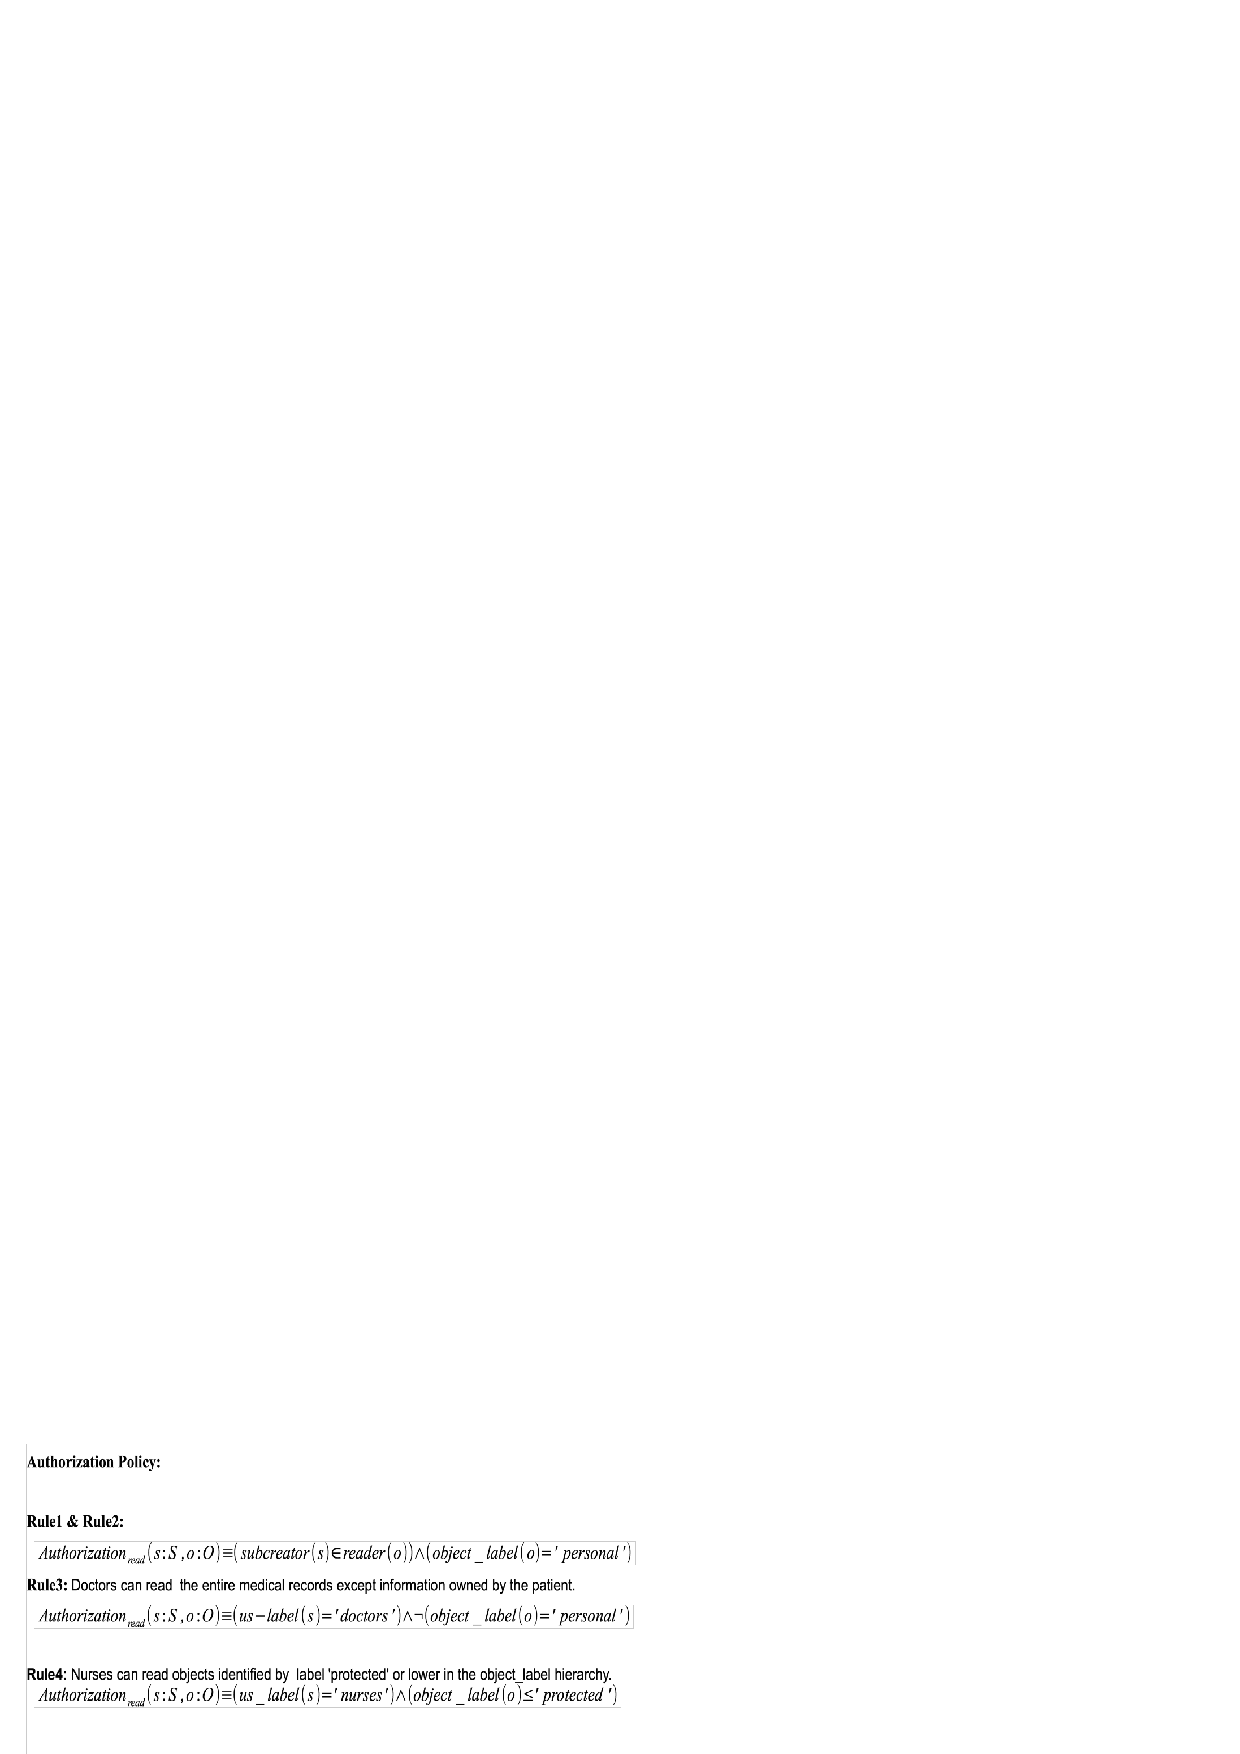
\includegraphics[width=0.5\textwidth]{eps/policy}
 \caption{Configured ABAC policy for given policy.}
\label {fig:policy} 
\end{figure}


Now, whenever a user having role doctor request to get the whole file, he would be able to access only the content as specified in listing \ref{request response} . Figure \ref{fig:policy} shows the configured ABAC policy used in our implementation.

\begin{listing}
\begin{minted}[frame=single,
               framesep=3mm,
               linenos=true,
               xleftmargin=21pt,
               tabsize=2]{js}
{
 "medical_record": { 
      "physical_exam": {
	  "appearance": "well developed",
	  "eyes": "conjunctiva"
	},
  "Medications": [
            "PRINIVIL TABS 20 MG ",
            "Last Refill: #30 x 2 "
        ]   
}  
}

\end{minted}
\caption{Content of  Medical Record Object as Accessed by a User Having Doctor Role} 
\label{request response}
\end{listing}


Again, we envision that it should  be possible to request the file by specifying a JSONPath along with the filename. For example, a requester having role 'doctor' should be able to access only   medication information by specifying a JSON path argument ("//medication") along with the request line. A hypothetical command for the above query would be 

\textbf{ Swift download container patient\_record.json --jsonpath="//medication" }


To sum up our proposal of Content Based Access Control, we want to achieve following:

\begin{figure}[h!] 
  \centering
    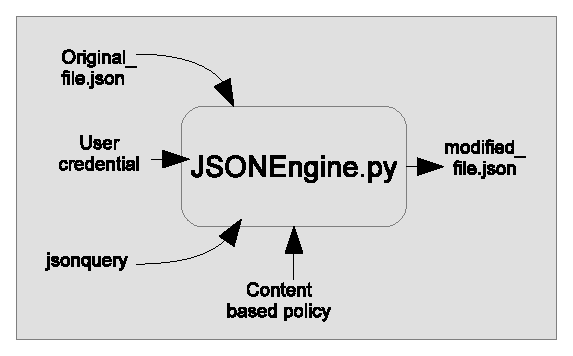
\includegraphics[width=0.3\textwidth]{eps/json_query_zap}
 \caption{The Skeleton for the CBAC zap.}
\label{fig:zappskeleton}
\end{figure}

\begin{enumerate}

  \item Attach policies with a file/object stored in Swift storage. The  file can be requested as it it, or it can be partially requested by specifying query parameter(JSONPath in our case) and instead of having the full content, the requester may get selective content based on his acting role. This case is explained in the above section. The skeleton for the to be developed ZeroVM application is shown in the figure \ref{fig:zappskeleton}



\end{enumerate}









